\section{Event}
\label{sec:Event}
%%%%%%%%%%%%%%%%%%%%%%%%%%%%%%%%%%%%%%%%%%%%%%%%%%%%%%%%
\begin{figure}[h!]
\begin{center}
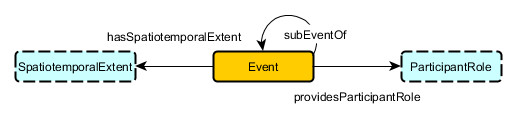
\includegraphics[width=.8\textwidth]{figures/event}
\end{center}
\caption{Schema Diagram for the Event pattern.}
\label{fig:Event}
\end{figure}
\subsection{Summary}
\label{sum:Event}
%%%%%%%%%%%%%%%%%%%%%%%%%%%%
The purpose of this pattern is to provide a minimalistic model of event where it is not always possible to separate its spatial and the temporal aspects, thus can model events that move or possess discontinuous temporal extent. Events, according to this model, have at least one participant, attached via a \textsf{ParticipantRole} (Section \ref{sec:ParticipantRole}). A more thorough examination of the pattern and some additional (optional) axioms can be found in \cite{event}. Some language is borrowed from \url{http://ontologydesignpatterns.org/wiki/Submissions:EventCore}.

%%%%%%%%%%%%%%%%%%%%%%%%%%%%%%%%%%%%%%%%%%%%%%%%%%%%%%%%
\subsection{Axiomatization}
\label{axs:Event}
%%%%%%%%%%%%%%%%%%%%%%%%%%%%
\begin{align}
% General Axioms
\textsf{subEventOf} \circ \textsf{subEventOf} &\sqsubseteq \textsf{subEventOf} \\
% Domain and Range Restrictions
\textsf{Event} &\sqsubseteq \text{=1} \textsf{hasSpatiotemporalExtent.SpatiotemporalExtent} \\
\textsf{Event} &\sqsubseteq \exists \textsf{providesParticipantRole.ParticipantRole} \\
\top &\sqsubseteq \forall \textsf{hasSpatiotemporalExtent.SpatiotemporalExtent} \\
\top &\sqsubseteq \forall \textsf{providesParticipantRole.ParticipantRole} \\
\exists \textsf{subEventOf.}\top &\sqsubseteq \textsf{Event} \\
\top &\sqsubseteq \forall \textsf{subEventOf.Event}
% Inverse Aliases (if any) 
\end{align}

%%%%%%%%%%%%%%%%%%%%%%%%%%%%%%%%%%%%%%%%%%%%%%%%%%%%%%%%
\subsection{Explanations}
\label{exp:Event}
%%%%%%%%%%%%%%%%%%%%%%%%%%%%
\begin{enumerate}
\item Role Chain: \textsf{subEventOf} is transitive.
\item \textsf{Event} has exactly one \textsf{SpatiotemporalExtent}. 
\item \textsf{Event} provides at least one \textsf{ParticipantRole}.
\item Range: the range of \textsf{hasSpatiotemporalExtent} is \textsf{SpatiotemporalExtent}.
\item Range: the range of \textsf{providesParticipantRole} is \textsf{ParticipantRole}.
\item Domain: the domain of \textsf{subEventOf} is \textsf{Event}.
\item Range: the range of \textsf{subEventOf} is \textsf{Event}.
\end{enumerate}

%%%%%%%%%%%%%%%%%%%%%%%%%%%%%%%%%%%%%%%%%%%%%%%%%%%%%%%%
\subsection{Remarks}
\label{rem:Event}
%%%%%%%%%%%%%%%%%%%%%%%%%%%%
It is also possible to equip the pattern with the following rule.
\begin{equation}
\textsf{Event}(x) \wedge \textsf{providesParticipantRole}(x,p) \wedge \textsf{subEventOf}(x,y) \rightarrow \textsf{providesParticipantRole}(y,p)
\end{equation}
This rule can be converted into OWL DL through \emph{rolification} \cite{KrisnadhiMH11}.This results in the following axioms.
\begin{align}
\textsf{Event} &\equiv \exists R_\textsf{Event}.\textsf{Self} \\
\textsf{subEventOf}^- \circ R_\textsf{Event} \circ \textsf{providesParticipantRole} &\sqsubseteq \textsf{providesParticipantRole}
\end{align} 
%%%%%%%%%%%%%%%%%%%%%%%%%%%%%%%%%%%%%%%%%%%%%%%%%%%%%%%%
\subsection{Competency Question}
\label{cqs:Event}
%%%%%%%%%%%%%%%%%%%%%%%%%%%%
\begin{enumerate}[CQ1.]
\item Where and when did the 1990 World Chess Championship Match take place?
\item Who were involved in the 1990 World Chess Championship Match?
\end{enumerate}
\newpage
%%%%%%%%%%%%%%%%%%%%%%%%%%%%%%%%%%%%%%%%%%%%%%%%%%%%%%%%
% End Section
%%%%%%%%%%%%%%%%%%%%%%%%%%%%%%%%%%%%%%%%%%%%%%%%%%%%%%%%
%%%%%%%%%%%%%%%%%%%%%%%%%%%%%%%%%%%%%%%%%%%%%%%%%%%%%%%%